% !TeX spellcheck = german
\documentclass[9pt,a4paper]{report}
\usepackage[T1]{fontenc}    
\usepackage[utf8]{inputenc} 
\usepackage{geometry}
\usepackage{wrapfig}
\geometry{
	letterpaper, % or a4paper
	total={6.5in, 8.75in}, % total width and height of the text area
	top=1.2in,
	left=1in,
	footskip=0.5in
}

\usepackage[bookmarks=true, pdfborder={0 0 0}]{hyperref}

\usepackage[ngerman]{babel,cleveref}

\hypersetup{
	colorlinks=true,      % Rahmen entfernen und Text einfärben
	linkcolor=blue,       % Farbe für interne Verweise (Tabellen, Kapitel, etc.)
	urlcolor=blue,        % Farbe für Web-Adressen
	citecolor=green!60!black % Farbe für Zitate (Dunkelgrün)
}


\usepackage{graphicx}

% --- CODE SETUP

\usepackage{listings}
\usepackage{xcolor}

\lstset{inputpath={{../02_Software/}}}

% Define colors for the code
\definecolor{codegreen}{rgb}{0,0.6,0}
\definecolor{codegray}{rgb}{0.5,0.5,0.5}
\definecolor{codepurple}{rgb}{0.58,0,0.82}
\definecolor{backcolour}{rgb}{0.95,0.95,0.92}

% Setup the style
\lstset{
	language=Python,
	backgroundcolor=\color{backcolour},   
	commentstyle=\color{codegreen},
	keywordstyle=\color{magenta},
	numberstyle=\tiny\color{codegray},
	stringstyle=\color{codepurple},
	basicstyle=\ttfamily\small,
	breakatwhitespace=false,         
	breaklines=true,                 
	captionpos=b,                    
	keepspaces=true,                 
	numbers=left,                    % Line numbers on the left
	numbersep=5pt,                  
	showspaces=false,                
	showstringspaces=false,
	showtabs=false,                  
	tabsize=2,
	literate={ö}{{\"o}}1 {ü}{{\"u}}1 {ä}{{\"a}}1 {ß}{{\"ss}}1 {°}{{\textdegree}}1
}

\title{ESP32 Wetter Station Teil 2}
\author{Anthony Timmel}

\begin{document}
	\maketitle
	\tableofcontents
	\cleardoublepage
	
	Im Rahmen des ersten Teils dieser Dokumentation setzen wir uns intensiv mit der initialen Aufgabenstellung aus dem Unterricht des Lernfeldes 7 (LF7) auseinander. Auf den nachfolgenden Seiten wird Ihnen das Projekt \textit{Wetterstation ESP32} in seiner zweiten Phase detailliert und in schriftlicher Form präsentiert, um einen fundierten Überblick über die Zielsetzung und den Aufbau zu geben.
	
	Diese Dokumentation ist der zweite Teil der Dokumentationsreihe, über den \textit{ESP32} als Wetterstation.
	
	\chapter{Grundlagen}
	Innerhalb des zweiten Teils, kommen neue softwarebasierte Technologien zum Einsatz. Damit, bei der Referenzierung auf diese Begriffe \& bei dem Ablauf der Beschreibung des Programmcodes keine Komplikationen in dem Verständniss des Ablaufs auftreten, werden die Begrifflichkeiten, im Unfang der zweiten Aufgabenstellung erklärt.
	Für eine detailiertere Beschreibung der einzelnen Begriffe, empfielt sich das Lesen der Beitrage auf \hyperref{https://www.hivemq.com}{hivemq}{HiveMQ}{HiveMQ}
	
	\section{Begriffe des MQTT-Protokolls}
	In den folgenden Sektionen, werden Ihnen folgende Begriffe erklärt. Dies geschieht innerhalb des Rahmens von \textit{Skript Teil 3}.
	
	\subsection{MQTT-Broker}
	Der MQTT-Broker ist vergleichbar mit der Poststation. Der Broker erhält Nachrichten von den Clients \& sendet diese an andere Clients weiter, die in diesen bestimmten Topics subscribed haben.
	
	\subsection{MQTT-Client}
	Der MQTT-Client ist der Part, der innerhalb von z.B. IoT-Geräten eingebaut ist \& für die Datenübertragung sowie Kommunikation verwendet wird. Der Client stellt eine Verbindung zum Broker her \& subscribed zu ausgewählten Topics \&/oder sendet ebenfalls auf diese Daten an den Broker zurück.
	
	\subsection{MQTT-Topic und dessen Grundregeln}
	Eine MQTT-Topic ist eine Art Channel für die Kommunikation. Diese können basierend auf Pfaden von einander getrennt werden. Dabei ermöglicht es einem, nur auf bestimmte Aktivitäten zu reagieren, anstatt die Nachrichten erst Clientseitig zu verwalten. Dies reduziert zum einen die Menge an Daten die versendet werden, ebenfalls benötigt der Client weniger Funktionalität bei der Nachrichtenpriorisierung \& Zuordnung, da er nur das Erhält, was er selbst gewählt hat.
	
	\subsection{Topic Wildcard einstufig und mehrstufig}
	In MQTT gibt es zwei verschiedene Arten von Topic-Wildcards.
	Die erste Variante sind die einstufigen Wildcards, in MQTT wird hierführ das \texttt{+} benutzt. Eine Wildcard könnte daher wie folgt aussehen \newline \texttt{abc/outlet01/+/audiQ3}. Die einstufige Wildcard würde nun alle Topics subscriben z.B. \newline (\texttt{abc/outlet01/alert0/audiQ3}, \texttt{abc/outlet01/alert1/audiQ3} usw.).
	
	Mehrstufige Topic Wildcards werden in MQTT mit dem \texttt{\#} deklariert. Hierbei muss jedoch die Wildcard als letzter Pfad Parameter gesetzt sein. \texttt{abc/outlet01/alert0/\#} währe daher eine \textbf{valide} Wildcard. \texttt{abc/outlet01/\#/audiQ3} ist hierbei eine \textbf{invalide} Wildcard
	
	\subsection{Stufenmodell Quality of Service (QoS)}
	Das Stufenmodell QoS ist für die Priorisierung von dem Datenverkehr im globalen \& privaten Netzwerk zuständig. Hierbei gibt es folgende 4 Stufen der Priorisierung.
	\newline
	\newline
	0-1 (Best Effort): Standarddatenverkehr (Web-Surfen, E-Mail).\newline 2-3 (Best Effort+): Höhere Priorität als Standard. \newline 4-5 (Echtzeit/Streaming): Reserviert für Video-Streaming, Telefonie (VoIP). Hier sind Verzögerungen (Jitter) und Paketverluste kritisch. \newline 6-7 (Netzwerksteuerung): Höchste Priorität, reserviert für Netzwerk-Routing-Protokolle
	
	\newpage
	\subsection{Last Will Testament}
	Last Will Testament (LWT) ist für das Verwalten von Topics ausschlaggebend. Hierbei sendet der Broker bei einem unerwarteten disconnect von einem Client, eine Nachricht an alle anderen Clients in dieser Topic.
	\begin{figure}[!h]
		\centering
		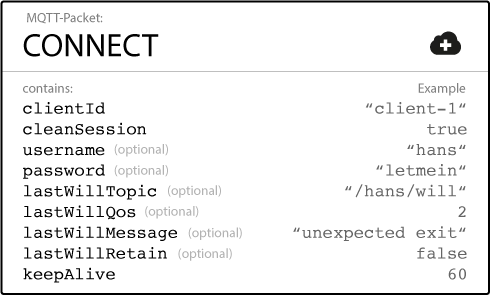
\includegraphics[width=0.7\linewidth]{assets/connect-msg-lwt}
		\caption[Last Will Message by HiveMQ]{Last Will Message im Connect Packet (Grafik von HiveMQ)}
		\label{fig:last-will-connect-message}
	\end{figure}
	\begin{figure}[!h]
		\centering
		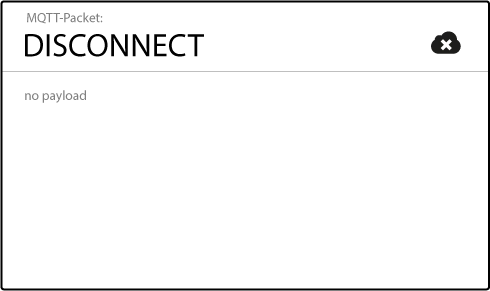
\includegraphics[width=0.7\linewidth]{assets/disconnect-msg-lwt}
		\caption[Last Will Message by HiveMQ]{Last Will Message beim Disconnect (Grafik von HiveMQ)}
		\label{fig:last-will-disconnect-msg}
	\end{figure}
	In dem ersten Bild sehen Sie das Connect MQTT-Packet. Innerhalb dieses gibt es den Parameter \texttt{lastWillMessage}, hier kann eine eigene Nachricht verfasst werden. Ebenfalls gibt es weitere Einstellungsmöglichkeiten für den LWT, wie z.B. in welcher Topic der LWT gesendet werden soll, oder in welcher Priorität \textit{QoS} die Nachricht versendet werden soll.
	
	
	\section{Verbindungsmanagement zwischen Client und Server}
	In den folgenden Sektionen, werden Ihnen folgende Begriffe erklärt. Dies geschieht innerhalb des Rahmens von \textit{Skript Teil 3}.
	
	\subsection{Retained Messages}
	Eine retained Message ist eine Nachricht, die auf dem Server (in unserem Fall Broker) gespeicherte Nachricht. Damit diese Nachricht gespeichert wird, muss die \texttt{retained}-Flag aktiv sein. Dann speichert der Broker vorübergehend die Nachricht für diese Topic inkl. QoS auf dem Server. Sobald sich ein neuer Client mit der Topic per Subscribe verbindet, erhält er diese Nachricht.
	
	\subsection{Persistent Sessions}
	Peristent Sessions haben Ähnlichkeiten zu den Retained Messages, erweitern jedoch den Funktionsrahmen um ein weiteres.
	Bei einer Persistent Session speichert der Server alle nicht zustellbaren Nachrichten an den Client in den subscribten Topics \& versucht es erneut, sobald der MQTT-Client wieder mit dem Broker verbunden ist. Damit der Broker überhaupt erstmal bescheid weiß, dass der Client eine Persistent Session erstellen möchte, muss dies bei dem Verbinden mit dem Broker, übermittelt werden. 
	
	\subsection{Keep Alive}
	Keep Alive ist eine Funktionalität um eine Verbindung mit dem Broker aufrecht zu erhalten, obwohl kein Nachrichtenaustausch zwischen Broker \& Client stattfindet. Diese Funktionalität kann ebenfalls bei dem erstellen des Clients eingestellt werden.
	
	\subsection{Web Sockets Transport}
	Web Sockets Transport ist eine Möglichkeit das MQTT Protokoll zu erweitern \& für die Browser möglich zu machen.
	Dabei wird das MQTT Protokoll mit dem WebSocket Protokoll erweitert, dadurch können Browser ebenfalls an einer Topic im MQTT-Broker subscriben \& die Daten verwalten.
	
	\section{Pub/Sub Messaging}
	Pub/Sub Messaging ist eine Protokollfamilie. Hierbei werden Nachrichten in sogenannten \textbf{Channeln} oder \textbf{Topics} versendet. Man könnte dies mit den verschiedenen Bereichen in einem Amt vergleichen, denn je nach Channel, geht die Nachricht an andere Empfänger über. Jedoch bleiben für den Clienten die Empfänger unbekannt.
	
	Pub/Sub ist ein serverbasierters Nachrichtenprotokoll, d.h. die Nachricht, die ein Client versendet, werden an einen Server gesendet. Dieser \textit{Verwaltet} die Eingehenden \& Ausgehenden Verbindungen, den andere Clients können sich an diese Topics anklinken. Dadurch wird die Nachricht, sobald diese bei dem Server ankommt, automatisch an diese Clienten versendet.
	\begin{figure}[!h]
		\centering
		\includegraphics[width=0.7\linewidth]{"assets/Berufsschule - Pub_Sub Messaging"}
		\caption[Grafik von Anthony Timmel]{Grafiische Darstellung des Pub/Sub Verfahrens}
		\label{fig:berufsschule-pubsub-messaging}
	\end{figure}
	In dieser Grafik sieht man zwei verschiedene \textbf{Publisher} Clients. Diese senden eine Nachricht auf \textbf{/order} \& \textbf{/inventory}. Beide senden die Nachricht mit dem Channel/Topic an den Pub/Sub Server. Hinter dem Pub/Sub Server befinden sich drei unterschiedliche Clients. Zwei dieser Clients hören auf Nachrichten innerhalb des \textbf{/order} Channels \& einer auf den \textbf{/inventory}. Die Verbindung zwischen Client \& Server bestehen aus WebSocket Verbindungen, damit der Server \& der Client sich gegenseitig Nachrichten zusenden zu können.
	
	\newpage
	\section{MQTT-Client}
	\begin{figure}[!h]
		\centering
		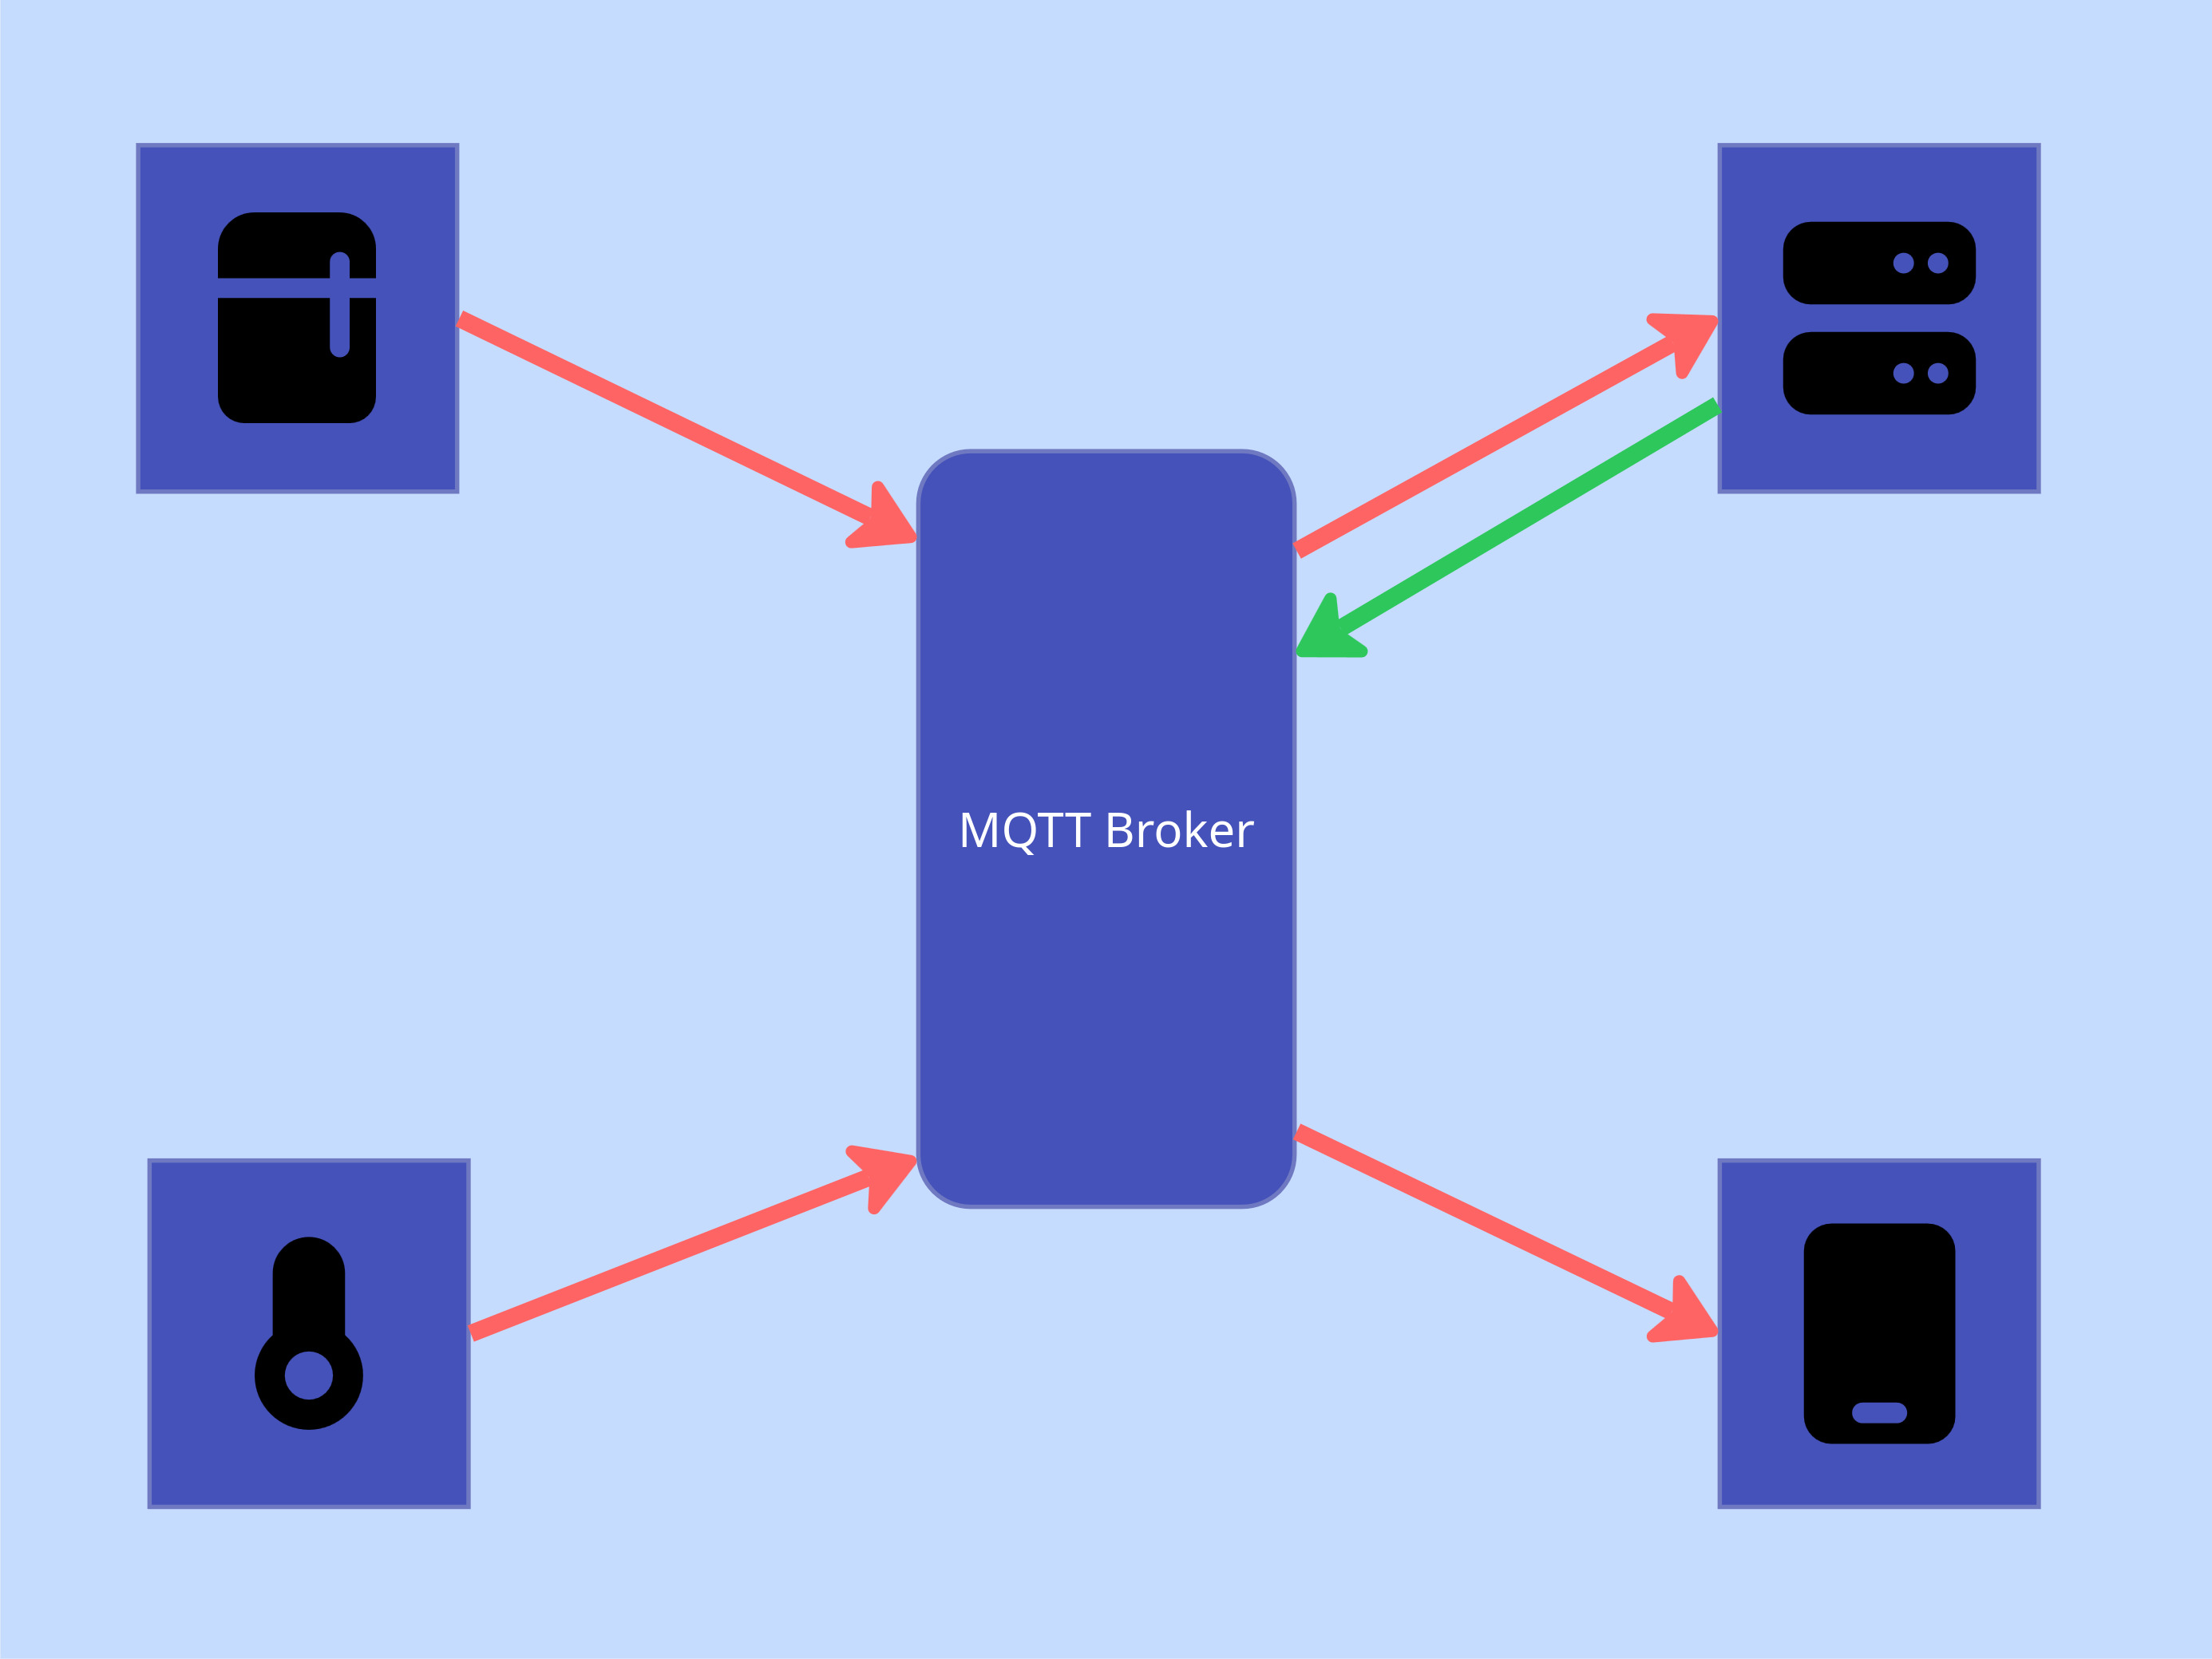
\includegraphics[width=0.7\linewidth]{assets/Berufsschule-MQTT}
		\caption[Grafik von Anthony Timmel]{Grafik von MQTT}
		\label{fig:berufsschule-mqtt}
	\end{figure}
	Diese Grafik verbildlicht die Kommunikation zwischen den einzelnen Geräten wie den Kühlschrank, Thermometer, Server \& einem Handy. Hierbei werden die Daten mithilfe von dem MQTT-Client an den Broker gesendet. Der Broker sendet diese Daten dann an alle Clienten, die den \textbf{Channel} subscribed haben.
	
	Innerhalb dieses zweiten Teils werden Daten an einen externen Dienst versendet. Dafür gibt es verschiedene Wege, diesen Prozess zu absolvieren. 
	
	Das MQTT-Protokoll ist ein klassiches Pub/Sub Modell in der IoT Welt.
	Hierbei agiert es als leichtgewichtiges Messaging Protokoll für die Übermittlung von Daten, von unseren Client an den Server.
	
	\chapter{Internetverbindung für den ESP32}
	Damit Daten überhaupt von dem ESP32 an den MQTT-Broker übermittelt werden können, benötigt der ESP32 eine Internetverbindung.
	
	Für die technische Umsetzung wurde sich auf die \hyperref{https://docs.micropython.org/en/v1.21.0/esp32/quickref.html#wlan}{ESP32\_Dokumentation}{esp32-wlan}{ESP32 WLAN Modul} Dokumentation bezogen.
	
	\section{Planung}
	Der ESP32 soll sich mit einem W-LAN AccessPoint in der Nähe verbinden \& dadurch eine internetfähige Verbindung aufbauen, damit später, eine Möglichkeit besteht, den MQTT-Broker zu erreichen.
	
	
	\section{Programmcode}
	
	\begin{lstlisting}
	import network
	
	wlan = network.WLAN(network.STA_IF)
	
	def do_connect():
		wlan.active(True)
		if not wlan.isconnected():
			print('connecting to network...')
			wlan.connect('FI24-Hotspot', 'BszWsw11#')
			while not wlan.isconnected():
				print("WLAN is not connected")
				pass
	
		print('network config:', wlan.ifconfig())
	
	do_connect()
	\end{lstlisting}
	
	Zuerst importieren wir das Modul \textbf{network}.
	In Zeile 3 deklarieren wir das WLAN-Modul des ESP32, indem wir aus dem Netzwerk-Modul die Klasse \textbf{WLAN} instanziieren. \texttt{network.STA\_IF} bedeutet hierbei, das wir es als Station Interface deklarieren, also ein stationärer Zugriffspunkt (Access Point).
	
	Damit wir später im Programmcode einfacher eine W-LAN Verbindung herstellen können, deklarieren wir die Funktion \texttt{do\_connect()}. Innerhalb des Funktionsbodies, aktivieren wir zuerst die WLAN-Funktionalität, damit wir uns später mit einem Access Point verbinden können. Wir überprüfen zuerst, ob wir mit einem Access-Point verbunden sind. Dies verhindert, dass wir die Verbindung zu dem Access-Point neu aufbauen, obwohl wir bereits eine Verbindung haben.
	
	In Zeile 9 verbinden wir uns mit dem definierten Access Point \& überprüfen in der while-Schleife dann so lange, ob die Verbindung erfolgreich war. Erst nach einer erfolgreichen Verbindung lassen wir die while-Schleife los \& geben die IP-Informationen in die Konsole aus.
	
	Damit die WLAN Verbindung initzialisiert werden kann, wird die Funktion \texttt{do\_connect()} aufgerufen.
	
	\chapter{MQTT-Client}
	
	\section{Planung}
	Der ESP32 soll bei einer internetfähigen Verbindung, sich mit dem MQTT-Broker verbinden \& pro Durchlauf die Daten an den Broker senden, über eine zuvor definierte Topic.
	
	\section{Programmcode}
	
	\begin{lstlisting}
	from umqtt.simple import MQTTClient
	
	client_id = "ESP_32_MQTT"
	server = "mosquitto.nodered-fi.ipv64.net"
	port = 0
	user = "FI"
	password = "FI"
	keepalive = 1
	mqtt_client = MQTTClient(client_id, server, port, user, password, keepalive=0, ssl=False, ssl_params={})
	
	def mqtt_connect():
		mqtt_client.connect()
		
	def send_mqtt_message(message):
		channel = "Met/FI/Timmel"
		mqtt_client.publish(channel, message)
	\end{lstlisting} 
	
	\chapter{Verarbeitung der Daten in NODE-RED}
	\section{MQTT-Client innerhalb von NODE-RED}
	Alle Daten kommen zuerst über einen MQTT-Client in Node-RED. Dieser Client ist an die selbe Topic subscribed, wie unser MQTT-Client für den ESP32 die Daten an den Broker sendet.
	
	
	\begin{figure}[h!]
		\centering
		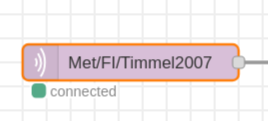
\includegraphics[width=0.3\linewidth]{assets/mqtt-client-node}
		\caption{}
		\label{fig:mqtt-client-node}
	\end{figure}
	Die Node \textit{mqtt in} representiert einen MQTT Client, mitdem wir in diesem Beispiel eine Topic subscriben \& die Daten anschließend innerhalb von Node-RED weiterverarbeiten.
	
	\begin{figure}[h!]
		\centering
		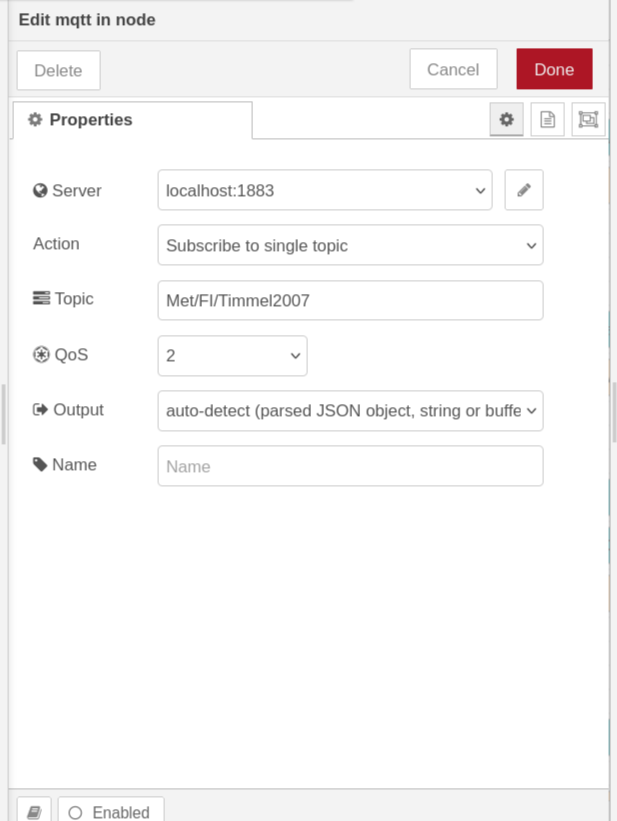
\includegraphics[height=0.3\textheight]{assets/mqtt-client-node-red-info}
		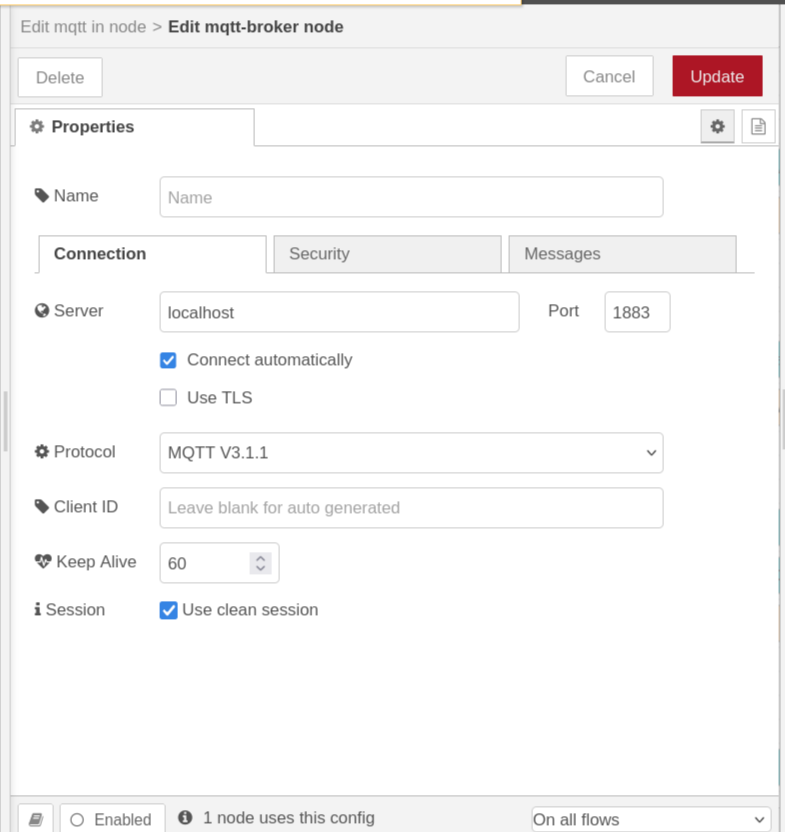
\includegraphics[height=0.3\textheight]{assets/mqtt-client-node-server}
		\caption{}
		\label{fig:mqtt-client-node-red-info}
	\end{figure}
	Bevor die Node jedoch die Daten empfangen kann, müssen wir diese zuvor Einrichten. Hierführ setzen wir die richtige Serverkonfiguration ein, in unserem Fall die IP \texttt{127.0.0.1} mit dem dazugehörigen Port \texttt{1883}. Ebenfalls müssen wir die Zugangsdaten für den MQTT-Broker übergeben, weshalb wir diese angeben müssen.
	Nachdem wir die Serververbindung zum Broker eingerichtet haben, setzen wir die passende Topic zum subscriben. Bestätigen die Änderungen und deployen den Flow.
	\newpage
	\begin{figure}[h!]
		\centering
		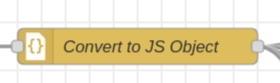
\includegraphics[width=0.3\linewidth]{assets/convert-node-to-jsobj}
		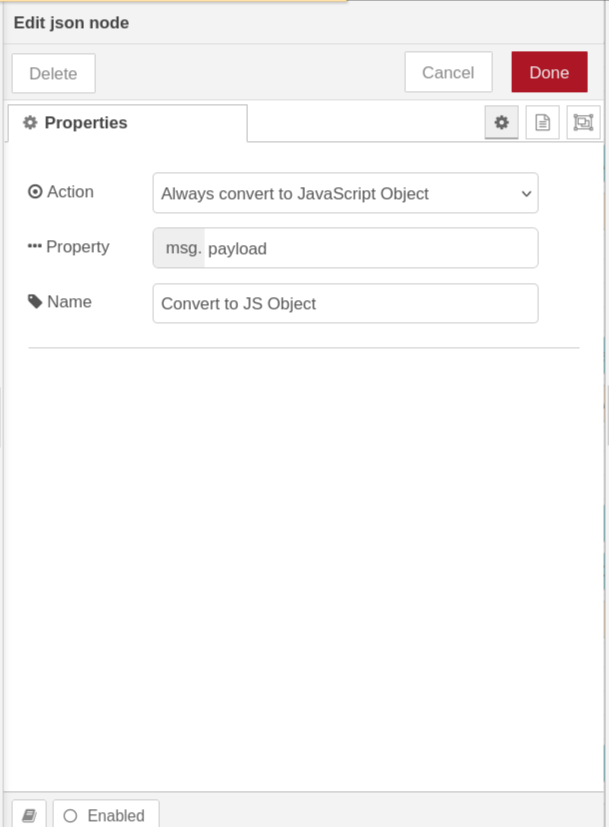
\includegraphics[height=0.3\textheight]{assets/convert-node-to-jsobj-view}
		\caption{}
		\label{fig:convert-node-to-jsobj}
	\end{figure}
	Mit der \textbf{Convert to JSON-Object} Node, konvertieren wir den JSON-String in ein valides JSON-Objekt.
	
	\newpage
	\section{Temperatur}
	\subsection{Vorbereitung der Daten für das UI}
	\begin{figure}[h!]
		\centering
		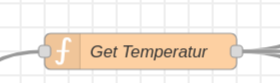
\includegraphics[width=0.3\linewidth]{assets/fun-to-temperature}
		\caption{}
		\label{fig:fun-to-temperature}
	\end{figure}
	Bevor wir die Daten für die Temperatur in die Visualisierung leiten können, müssen wir zuvor die richtigen Daten zuweisen.
	
	\begin{lstlisting}
	msg.payload = msg.payload.Temperatur;
	
	return msg;
	\end{lstlisting}
	Mithilfe dieses JavaScript Codes setzen wir die \texttt{msg.payload} Variable auf den Temperatur Wert, den wir zuvor erhalten haben.
	
	\subsection{UI Template für aktuelle Daten}
	\lstinputlisting[language=HTML]{../02_Software/templates/temperature/current.html}
	
	\subsection{UI Template für historie Daten}
	\lstinputlisting[language=HTML]{../02_Software/templates/temperature/history-converter.js}
	\lstinputlisting[language=HTML]{../02_Software/templates/temperature/history.html}
	\newpage
	\section{Luftfeuchtigkeit}
	\subsection{Vorbereitung der Daten für das UI}
	\begin{figure}[h!]
		\centering
		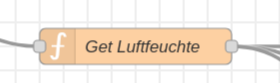
\includegraphics[width=0.3\linewidth]{assets/fun-to-humidity}
		\caption{}
		\label{fig:fun-to-humid}
	\end{figure}
	Bevor wir die Daten für die Luftfeuchtigkeit in die Visualisierung leiten können, müssen wir zuvor die richtigen Daten zuweisen.
	
	\begin{lstlisting}
		msg.payload = msg.payload.Luftfeuchtigkeit;
		
		return msg;
	\end{lstlisting}
	Mithilfe dieses JavaScript Codes setzen wir die \texttt{msg.payload} Variable auf den Luftfeuchtigkeit's Wert, den wir zuvor erhalten haben.
	
	\subsection{UI Template für aktuelle Daten}
	\lstinputlisting[language=HTML]{../02_Software/templates/humidity/current.html}
	
	\subsection{UI Template für historie Daten}
	\lstinputlisting[language=HTML]{../02_Software/templates/humidity/history-converter.js}
	\lstinputlisting[language=HTML]{../02_Software/templates/humidity/history.html}
	
	\newpage
	\section{Bewegung}
	\subsection{Vorbereitung der Daten für das UI}
	\begin{figure}[h!]
		\centering
		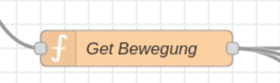
\includegraphics[width=0.3\linewidth]{assets/fun-to-motion}
		\caption{}
		\label{fig:fun-to-motion}
	\end{figure}
	Bevor wir die Daten für die Bewegung in die Visualisierung leiten können, müssen wir zuvor die richtigen Daten zuweisen.
	
	\begin{lstlisting}
		msg.payload = msg.payload.Luftfeuchtigkeit;
		
		return msg;
	\end{lstlisting}
	Mithilfe dieses JavaScript Codes setzen wir die \texttt{msg.payload} Variable auf den Bewegung Wert, den wir zuvor erhalten haben.
	
	\subsection{UI Template für aktuelle Daten}
	\lstinputlisting[language=HTML]{../02_Software/templates/motion/current.html}
	
	\subsection{UI Template für historie Daten}
	\lstinputlisting[language=HTML]{../02_Software/templates/motion/history-converter.js}
	\lstinputlisting[language=HTML]{../02_Software/templates/motion/history.html}
	\newpage
	\section{Helligkeit}
	\subsection{Vorbereitung der Daten für das UI}
	\begin{figure}[h!]
		\centering
		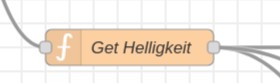
\includegraphics[width=0.3\linewidth]{assets/fun-to-luminance}
		\caption{}
		\label{fig:fun-to-luminance}
	\end{figure}
	Bevor wir die Daten für die Helligkeit in die Visualisierung leiten können, müssen wir zuvor die richtigen Daten zuweisen.
	
	\begin{lstlisting}
		msg.payload = msg.payload.Helligkeit;
		
		return msg;
	\end{lstlisting}
	Mithilfe dieses JavaScript Codes setzen wir die \texttt{msg.payload} Variable auf den Helligkeit Wert, den wir zuvor erhalten haben.
	
	\subsection{UI Template für aktuelle Daten}
	\lstinputlisting[language=HTML]{../02_Software/templates/luminance/current.html}
	
	\subsection{UI Template für historie Daten}
	\lstinputlisting[language=HTML]{../02_Software/templates/luminance/history-converter.js}
	\lstinputlisting[language=HTML]{../02_Software/templates/luminance/history.html}
	
	\chapter{Ganzer Programmcode für ESP32}
	\lstinputlisting[language=python]{../02_Software/boot.py}
	
\end{document}